\documentclass[xcolor={dvipsnames}]{beamer}
\mode<presentation>
{
  \usetheme{Antibes}      % or try Darmstadt, Madrid, Warsaw, ...
  \usecolortheme{dolphin} % or try albatross, beaver, crane, ...
  \usefonttheme{professionalfonts}  % or try serif, structurebold, ...
  \setbeamertemplate{navigation symbols}{}
  \setbeamertemplate{caption}[numbered]
} 
\usepackage[utf8]{inputenc}
\usepackage[english]{babel}
\usepackage{multirow}
\usepackage{mathrsfs}
\usepackage{subfigure}
\usepackage{amsmath}
\usepackage{amssymb} 
\usepackage{multirow}
\usepackage{graphicx}
\usepackage{indentfirst}
\usepackage{amsfonts}
\usepackage{algorithm}  
\usepackage{algorithmicx}  
\usepackage{algpseudocode}
\usepackage{titlesec}
\usepackage{enumitem}
\usepackage{tasks}
\usepackage{xcolor}
\usepackage{tikz}
\usepackage{graphicx,wrapfig,lipsum}
\usepackage{color}
\graphicspath{{/D:/fh/JI/latex/VE230 slides}}
\usepackage{amsmath}
\title[VE230 RC slides Final RC slides]{VE230 Final RC slides}
\author{han.fang }
\date{\today}


\begin{document}
\begin{frame}
\titlepage
\end{frame}

\begin{frame}{Review of Static Case}
	\begin{table}
		\centering
		\begin{tabular}{|l|c|c|}
\hline Fundamental Relations & Electrostatic & Magnetostatic \\
& Model & Model \\
\hline \multirow{2}{*} { Governing equations } & $\nabla \times \mathbf{E}=0$ & $\nabla \cdot \mathbf{B}=0$ \\
& $\nabla \cdot \mathbf{D}=\rho$ & $\nabla \times \mathbf{H}=\mathbf{J}$ \\
\hline Constitutive relations  & $\mathbf{D}=\epsilon \mathbf{E}$ & $\mathbf{H}=\frac{1}{\mu} \mathbf{B}$ \\
\hline
\end{tabular}
	\end{table}
	In static case, \textbf{E}, \textbf{B} can exist together(In a conducting medium), but they won’t influence each other.
\end{frame}


\begin{frame}{Faraday’s Law of Electromagnetic Induction}
\begin{itemize}
	\item Content: The relationship between induced emf and the negative rate of change of flux linkage.
	\item Expressions:
	$$
	\begin{gathered}
	\nabla \times \mathbf{E}=-\frac{\partial \mathbf{B}}{\partial t} \\
	\oint_{c} \mathbf{E} \cdot d \ell=-\int_{s} \frac{\partial \mathbf{B}}{\partial t} \cdot d \mathbf{s}\\
	\end{gathered}
	$$
\end{itemize}

\end{frame}

\begin{frame}{Static Circuit in a Time-varying Magnetic Field}
	If we assign emf $V=\oint_{c} \mathbf{E} \cdot d \ell$ and magnetic flux $\Phi=\int_{S} \mathbf{B} \cdot d \mathbf{s}$, we can get the Faraday’s Law
	$$V=-\frac{d \Phi}{d t}$$
	If there are N turns wires, the total magnetic flux is $N \Phi, V=-N \frac{d \Phi}{d t}$.
	
	\textbf{Lenz’s Law}: The induced emf will cause a current to flow in the closed loop in such a direction as to oppose the change in the linking magnetic flux.
	
	
\end{frame}


\begin{frame}{Transformer}
\textbf{Transformer}: two or more coils coupled magnetically through a common ferromagnetic core.
\begin{figure}[H]
	\centering
	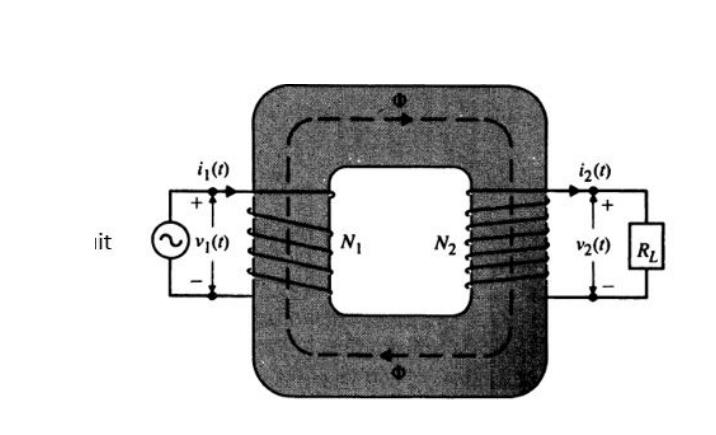
\includegraphics[width=0.7\linewidth]{8_1.png}
\end{figure}
The general equation is
$$N_{1} i_{1}-N_{2} i_{2}=\frac{\ell}{\mu S} \Phi$$
\end{frame}

\begin{frame}{Transformer}
\begin{itemize}
	\item \textbf{Ideal Transformer:} $\mu\rightarrow\infty$, and then we can get
	$$\frac{i_{1}}{i_{2}}=\frac{N_{2}}{N_{1}}$$
	Given Faraday’s Law, We get ratio of emf as
	$$\frac{V_{1}}{V_{2}}=\frac{N_{1}}{N_{2}}$$
	If we have RL in secondary circuit, we can see source Resistor $R_1=\frac{V_1}{i_1}$ as
	$$\left(R_{1}\right)_{e f f}=\left(\frac{N_{1}}{N_{2}}\right)^{2} R_{L}$$
\end{itemize}
\end{frame}
\begin{frame}{Moving Conductor in Static Magnetic field}
	\begin{itemize}
		\item \textbf{Working process:} $F_{m}=q \mathbf{u} \times \mathbf{B} \rightarrow$ positive and negative charge move to opposite direction $\rightarrow$ built induced Electric field $E_{\text {induced }}=-\mathbf{u} \times \mathbf{B} \rightarrow$  Other charges in equilibrium (they won’t move along the bar)
		\item \textbf{Motional EMF} $\mathcal{V}^{\prime}=\oint_{c}(\mathbf{u} \times \mathbf{B}) \cdot d \ell$.
	\end{itemize}
\end{frame}
\begin{frame}{Moving Circuit in a Time-varying Magnetic Field}
\begin{itemize}
	\item Lorentz’s force equation: $\mathbf{F}=q(\mathbf{E}+\mathbf{u} \times \mathbf{B})$.
	\item Effective electric field E': If an observer have the same movement with q, Lorentz’s force on q can be seen as effective electric field
	$$\mathbf{E}^{\prime}=\mathbf{E}+\mathbf{u} \times \mathbf{B}$$
	\item General form of Faraday’s law:
	$$\oint_{C} \mathbf{E}^{\prime} \cdot d \ell=-\int_{S} \frac{\partial \mathbf{B}}{\partial t} \cdot d \mathbf{s}+\oint_{C}(\mathbf{u} \times \mathbf{B}) \cdot d \ell$$
	
\end{itemize}
\end{frame}
\begin{frame}{Moving Conductor in Static Magnetic field}
\begin{itemize}
	\item Where left side talks about emf induced in a moving frame of reference, and on right side, transformer emf equals to
	$$V=-\int_{S} \frac{\partial \mathbf{B}}{\partial t} \cdot d \mathbf{s}$$
	and motional emf equals to
	$$V=\oint_{C}(\mathbf{u} \times \mathbf{B}) \cdot d l$$
	\item Faraday’s Law also works a moving circuit. If we use $V=\oint_{C} \mathbf{E}^{\prime} \cdot d \mathbf{l}$, then 
	$$V=-\frac{d}{d t} \int_{S} \mathbf{B} \cdot d \mathbf{s}=-\frac{d \Phi}{d t}$$
\end{itemize}
\end{frame}
\begin{frame}{Maxwell’s Equation}
\[
\begin{array}{|ccc|}
\hline \text { Differential Form } & \text { Integral Form } & \text { Significance } \\
\hline \nabla \times \mathbf{E}=-\frac{\partial \mathrm{B}}{\partial t} & \oint_{c} \mathbf{E} \cdot d \ell=-\frac{d \Phi}{d t} & \text { Faraday's law } \\
\nabla \times \mathbf{H}=\mathbf{J}+\frac{\partial \mathbf{D}}{\partial t} & \oint_{c} \mathbf{H} \cdot d \ell=I+\int_{s} \frac{\partial \mathrm{D}}{\partial t} \cdot d \mathbf{s} & \text { Ampère's circuital law } \\
\nabla \cdot \mathbf{D}=\rho & \oint_{s} \mathbf{D} \cdot d \mathbf{s}=Q & \text { Gauss's law } \\
\nabla \cdot \mathbf{B}=0 & \oint_{s} \mathbf{B} \cdot d \mathbf{s}=0 & \text { No isolated magnetic charge } \\
\hline
\end{array}
\]
Other useful equations:
\[
\begin{array}{c}
\nabla \cdot \mathbf{J}=\frac{\partial \rho}{\partial t} \\
\mathbf{H}=\mathbf{B} / \mu \\
\mathbf{D}=\epsilon \mathbf{E}
\end{array}
\]

\end{frame}
\begin{frame}{Potential Function}
\begin{itemize}
\item Electric Field time-varying field:
$$E=-\nabla V-\frac{\partial \mathbf{A}}{\partial t}$$
where  $-\nabla V $ comes from charge distribution, and  $-\frac{\partial \mathbf{A}}{\partial t}$  comes from time-varying current. Strictly speaking,  $\mathrm{V}$  and $ \mathrm{A} $ are calculated by the Poisson's Equation in time varying field.
\item Quasi-static fields: If  $\rho$  and  $\mathbf{J}$  vary slowly with time and the range of  $\mathrm{R}$  is small in comparison with the wavelength ( low frequency, long wavelength), We can use below 2 equations to find quasi-static fields.
\[
\begin{aligned}
V &=\frac{1}{4 \pi \epsilon_{0}} \int_{V^{\prime}} \frac{\rho}{R} d v^{\prime} \\
\mathbf{A} &=\frac{\mu_{0}}{4 \pi} \int_{V^{\prime}} \frac{\mathbf{J}}{R} d v^{\prime}
\end{aligned}
\]
\end{itemize}
\end{frame}
\begin{frame}{Potential Function}
\begin{itemize}
	\item Non-homogeneous wave equation for vector potential:
	
	if we choose divergence and curl of \textbf{A} as 
	\[
	\begin{array}{c}
\nabla \cdot \mathbf{A}+\mu \epsilon \frac{\partial V}{\partial t} \\
B=\nabla \times \mathbf{A}
\end{array}
	\]
	which is also called Lorentz condition, we can find the nonhomogeneous wave equations as
	$$\nabla^{2} \mathbf{A}-\mu \epsilon \frac{\partial^{2} \mathbf{A}}{\partial t^{2}}=-\mu \mathbf{J}$$
	\item Non-homogeneous wave equation for Scalar Potential V:
	$$\nabla^{2} V-\mu \epsilon \frac{\partial^{2} V}{\partial t^{2}}=-\frac{\rho}{\epsilon}.$$
\end{itemize}
\end{frame}
\begin{frame}{Electromagnetic Boundary Condition}
General Boundary Condition Equations:
\[
\begin{array}{c}
E_{1 t}=E_{2 t}(\mathrm{~V} / \mathrm{m}) \\
\mathbf{a}_{n 2} \times\left(\mathbf{H}_{1}-\mathbf{H}_{2}\right)=\mathbf{J}_{s} \quad(\mathrm{~A} / \mathrm{m}) \\
\mathbf{a}_{n 2} \cdot\left(\mathbf{D}_{1}-\mathbf{D}_{2}\right)=\rho_{s} \quad\left(\mathrm{C} / \mathrm{m}^{2}\right) \\
B_{1 n}=B_{2 n}(\mathrm{~T})
\end{array}
\]
Note that (1)(4) are equivalent and (2)(3) are equivalent. Since divergence equation can be derived
from curl equations with continuity equation.
\end{frame}
\begin{frame}{Interface between two lossless Linear Media}
\begin{itemize}
	\item lossless media: $\sigma=0$, then we can get J = 0.
	\item Usually, no free charge and no surface currents at the interface of two lossless. $\left(\rho_{s}=0, \mathbf{J}_{\mathbf{s}}=0\right)$.
	\item Boundary condition:
	\[
	\begin{array}{l}
E_{1 t}=E_{2 t} \rightarrow \frac{D_{1 t}}{D_{2 t}}=\frac{\epsilon_{1}}{\epsilon_{2}} \\
H_{1 t}=H_{2 t} \rightarrow \frac{B_{1 t}}{B_{2 t}}=\frac{\mu_{1}}{\mu_{2}} \\
D_{1 n}=D_{2 n} \rightarrow \epsilon_{1} E_{1 n}=\epsilon_{2} E_{2 n} \\
B_{1 n}=B_{2 n} \rightarrow \mu_{1} H_{1 n}=\mu_{2} H_{2 n}
\end{array}
	\]
\end{itemize}
\end{frame}
\begin{frame}{Interface between a Dielectric and a perfect conductor}
\begin{itemize}
	\item perfect conductor: $\sigma\rightarrow\infty$, then we know $\mathbf{E}_{inside}=0$, the charge only exists on the surface.
	\item $\mathbf{D}, \mathbf{B}, \mathbf{H} = 0$ for point inside a conductor.
	\item Boundary condition equation (2 is perfect):
	$$
\begin{array}{|rc|}
\hline \text { On the Side of Medium 1 } & \text { On the Side of Medium 2 } \\
\hline E_{1 t}=0 & E_{2 t}=0 \\
\mathbf{a}_{n 2} \times \mathbf{H}_{1}=\mathbf{J}_{s} & H_{2 t}=0 \\
\mathbf{a}_{n 2} \cdot \mathbf{D}_{1}=\rho_{s} & D_{2 n}=0 \\
B_{1 n}=0 & B_{2 n}=0 \\
\hline
\end{array}
$$
\end{itemize}
\end{frame}
\begin{frame}{solutions for wave equations for potentials}
The calculation process is on the textbook.
\begin{itemize}
	\item for given charge and current distribution $\rho$ and $\textbf{J}$,in order to get the $\textbf{E}$, $\textbf{B}$, we firstly need to
find solutions for $\textbf{A}$, $\textbf{V}$ in nonhomogeneous wave equation.
\item solution for scalar potential:
$$
V(R, t)=\frac{1}{4 \pi \epsilon} \int_{V}, \frac{\rho(t-R / u)}{R} d v^{\prime}
$$
It takes time $R/u$ for the effect of $\rho$ to be felted at the distance $R$, which means there is time retardation $\Delta t=R/u$ from $\rho$ to $V$.
\item solution for vector potential:
$$
\mathbf{A}(R, t)=\frac{\mu}{4 \pi} \int_{V}, \frac{\mathbf{J}(t-R / u)}{R} d v^{\prime} \quad(\mathbf{W} b / \mathrm{m})
$$
\end{itemize}
\end{frame}
\begin{frame}{Source-Free Wave Equations in simple nonconducting media}
\begin{itemize}
	\item Source-free; $\rho =0,\mathbf{J}=0$.
	\item In a simple nonconducting media: $\epsilon,\mu$ are constant, $\sigma = 0$
	\item Rewrite the Maxwell Equations:
	$$
\begin{aligned}
\nabla \times \mathbf{E} &=-\mu \frac{\partial \mathbf{H}}{\partial t} \\
\nabla \times \mathbf{H} &=\epsilon \frac{\partial \mathbf{E}}{\partial t} \\
\nabla \cdot \mathbf{E} &=0 \\
\nabla \cdot \mathbf{H} &=0
\end{aligned}
$$
\item Wave Equations for \textbf{E}, \textbf{H} can be found directly.
$$
\begin{aligned}
&\nabla^{2} \mathbf{E}-\frac{1}{u^{2}} \frac{\partial^{2} \mathbf{E}}{\partial t^{2}}=0 \\
&\nabla^{2} \mathbf{H}-\frac{1}{u^{2}} \frac{\partial^{2} \mathbf{H}}{\partial t^{2}}=0
\end{aligned}
$$
\end{itemize}
\end{frame}
\begin{frame}{Time Harmonic Electromagnetic}
\begin{itemize}
	\item Time harmonic Vector Phasor: $$
\mathbf{E}(x, y, z, t)=\operatorname{Re}\left[\mathbf{E}(x, y, z) e^{j w t}\right]
$$

Different or integrate it, we can find
$$
\begin{aligned}
&\partial \mathbf{E}(x, y, z, t) / \partial t=j \omega \mathbf{E}(x, y, z) \\
&\int \mathbf{E}(x, y, z, t) d t=\mathbf{E}(x, y, z) / j \omega
\end{aligned}
$$
\item Revised Maxwell Equation
$$
\begin{gathered}
\nabla \times \mathbf{E}=-j \omega \mu \mathbf{H} \\
\nabla \times \mathbf{H}=\mathbf{J}+j \omega \epsilon \mathbf{E} \\
\nabla \cdot \mathbf{E}=\rho / \epsilon \\
\nabla \cdot \mathbf{H}=0
\end{gathered}
$$
\end{itemize}
\end{frame}
\begin{frame}{Time Harmonic Electromagnetic}
\begin{itemize}
	\item Time harmonic wave equations:
	$$
\begin{aligned}
&\nabla^{2} V+k^{2} V=-\frac{\rho}{\epsilon} \\
&\nabla^{2} \mathbf{A}+k^{2} \mathbf{A}=-\mu \mathbf{J} \\
&\text { where } \quad k=\omega \sqrt{\mu \epsilon}=\frac{\omega}{u}=2 \pi / \lambda
\end{aligned}
$$
\item Phasor solutions:
$$
\begin{aligned}
V(R) &=\frac{1}{4 \pi \epsilon} \int_{V}, \frac{\rho e^{-j k R}}{R} d v^{\prime} \quad(V) \\
\mathbf{A}(R) &=\frac{\mu}{4 \pi} \int_{V^{\prime}} \frac{\mathbf{J} e^{-j k R}}{R} d v^{\prime} \quad(\mathbf{W b} / \mathrm{m})
\end{aligned}
$$
Note that $k R=2 \pi \frac{R}{\lambda}<<1$ when $R<<\lambda$.
\end{itemize}
\end{frame}
\begin{frame}{Procedure for determining E and H}
\begin{itemize}
	\item Find V and A by
	$$
V(R)=\frac{1}{4 \pi \epsilon} \int_{V}, \frac{\rho e^{-j k R}}{R} d v^{\prime} \quad \mathbf{A}(R)=\frac{\mu}{4 \pi} \int_{V^{\prime}} \frac{\mathbf{J} e^{-j k R}}{R} d v^{\prime}
$$
\item Find B and E by
$$
\mathbf{E}(R)=-\nabla V-j \omega \mathbf{A} \quad \mathbf{B}(R)=\nabla \times \mathbf{A}
$$
\item Find Instantaneous E(t) and B(t) by
$$
\mathbf{E}(R, t)=\mathcal{R} e\left[\mathbf{E}(R) e^{j \omega t}\right] \quad \mathbf{B}(R, t)=\mathcal{R} e\left[\mathbf{B}(R) e^{j \omega t}\right]
$$
\end{itemize}
\end{frame}
\begin{frame}{Source-Free Fields in non-conducting Simple Media}
\begin{itemize}
	\item Find Wave function given previous section
	$$
\nabla^{2} \mathbf{E}-\frac{1}{u^{2}} \frac{\partial^{2} \mathbf{E}}{\partial t^{2}}=0 \quad \nabla^{2} \mathbf{H}-\frac{1}{u^{2}} \frac{\partial^{2} \mathbf{H}}{\partial t^{2}}=0
$$
\item Find homogeneous equations in phasor form:
$$
\nabla^{2} \mathbf{E}+k^{2} \mathbf{E}=0 \quad \nabla^{2} \mathbf{H}+k^{2} \mathbf{H}=0
$$
If medium is conducting, We use $\nabla \times \mathbf{H}=j \omega \epsilon_{c} \mathbf{E}$ where complex permitivity $\epsilon_{c}=\epsilon-j \frac{\sigma}{\omega}(F / m)$.
\end{itemize}

\end{frame}
\begin{frame}{Flow of Electromagnetics Power and the Poynting Vector}
Power flow per unit area, Poynting vector, $\vec{\mathcal{P}}$ is defined as:
$$
\mathcal{P} = \vec{E}\times\vec{H}
$$

Poynting vector is a power density vector associated with an electromagnetics field. 

Poynting's theorem: the surface integral of $\mathcal{P}$ over a closed surface, equals the power leaving the enclosed volume, that is,

$$
\begin{aligned}
    &-\oint_S\mathcal{P}\cdot d\vec{s} = - \oint_S(\vec{E}\times\vec{H})\cdot d\vec{s} \\
    &= \frac{\partial}{\partial t} \int_V\left(\frac{1}{2}\epsilon E^2 + \frac{1}{2} \mu H^2\right) dv + \int_V \sigma E^2 dv\\
    & = \frac{\partial}{\partial t}\int_V(w_e + w_m)dv + \int_V p_\sigma dv
\end{aligned}
$$
\end{frame}
\begin{frame}{Flow of Electromagnetics Power and the Poynting Vector}
In the previous slides,
$$
w_e = \frac{1}{2}\epsilon E^2 = \frac{1}{2}\vec{E}\cdot\vec{E^*} = \text{Electric energy density}
$$

$$
w_m = \frac{1}{2}\mu H^2 = \frac{1}{2}\mu \vec{H}\cdot\vec{H^*} = \text{Magnetic energy density}
$$

$$
p_\sigma = \sigma E^2 = J^2/\sigma = \sigma \vec{E}\cdot\vec{E^*} = \vec{J}\cdot\vec{J^*}/\sigma = \text{Ohmic power density}
$$
If the region is loseless ($\sigma = 0$), 
$$
\text{total power flow in} = \text{rate of increase of the stored electric and magnetic energies}
$$,

moreover, for static situation, $w_e$ and $w_m$ vanish, the total power flowing into the closed surface equals to the ohmic power (usually heat) dissipated in the enclosed volume.

\end{frame}
\end{document}